\section{V\_sample: An incoherent scatterer, the V-sample}
\label{s:v_sample}
\index{Samples!Incoherent isotropic scatterer (Vanadium)}
\index{Incoherent elastic scattering}

\component{V\_sample}{System}{$r_{\rm i}$, $r_{\rm o}$, $h$, $r_{\rm foc}$, $x_{\rm target}$, $y_{\rm target}$, $z_{\rm target}$}{$w_x$, $h_y$, $t_z$, $w_{\rm focus}, h_{\rm focus}$, $w_{\rm foc, angle}$, $h_{\rm foc, angle}$, \\ $\sigma_{\rm abs}$, $\sigma_{\rm inc}$, $V_0$, $f_{\rm pack}$, target\_index}{validated}

A sample with incoherent scattering, e.g. vanadium, is frequently used for
calibration purposes, as this gives an isotropic, elastically scattered beam.

The component {\bf V\_sample}
has {\em only} absorption and incoherent elastic scattering.
For the sample geometry, we default use a
hollow cylinder (which has the solid cylinder as a limiting case).
The sample dimensions are: Inner radius $r_{\rm i}$,
outer radius $r_{\rm o}$, and height $h$, see figure \ref{f:v-sample}.
\begin{figure}
  \begin{center}
    \psfrag{ri}{$r_i$}
    \psfrag{ro}{$r_o$}
    \psfrag{h}{$h$}
    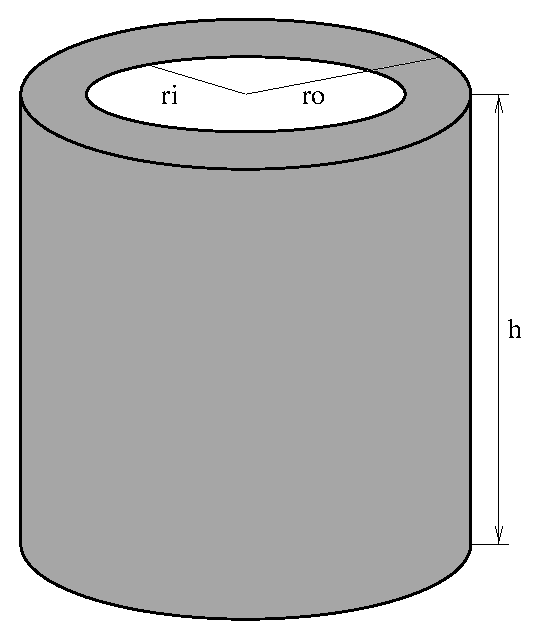
\includegraphics[width=0.3\textwidth]{figures/vsample.eps}
  \end{center}
\caption{The geometry of the hollow-cylinder vanadium sample.}
\label{f:v-sample}
\end{figure}

Alternatively, the sample geometry can be made rectangular
by specifying the width, $w_x$, the height, $h_y$, and the thickness, $t_z$.

The incoherent and absorption cross sections for V are default
for the component. For other choices, the
parameters $\sigma_{\rm inc}$, $\sigma_{\rm abs}$,
and the unit cell volume $V_0$ should be specified.
For a loosely packed sample, also the packing factor, $f_{\rm pack}$
can be specified (default value of 1).

\subsection{Physics and algorithm}

The incoherent scattering gives
a uniform angular distribution of the scattered
neutrons from each nucleus: $\gamma(\Omega) = 1/4\pi$.
For the focusing we choose to have a uniform distribution on
a target sphere of radius $r_{\rm foc}$, at the position
$(x_{\rm target},y_{\rm target},z_{\rm target})$
in the local coordinate system.
This gives an angular distribution (in a small angle approximation)
of
\begin{equation}
g(\Omega) = \frac{1}{4\pi}
  \frac{x_{\rm t}^2+y_{\rm t}^2+z_{\rm t}^2}{(\pi r_{\rm t}^2)}.
\end{equation}

The focusing can alternatively be performed on a rectangle with dimensions
$w_{\rm focus}$, $h_{\rm focus}$, or uniformly in angular space
(in a small-angle approximation),
using $w_{\rm foc, angle}$, $h_{\rm foc, angle}$.
The focusing location can be picked to be a downstream component by
specifying \\
\verb+target_index+.

When calculating the neutron path length within
the cylinder, the kernel function \\
\verb+cylinder_intersect+
is used twice, once for the outer radius and once
for the inner radius.

Multiple scattering is not included in this component. To obtain
intensities similar to real measured ones, we therefore do not
take attenuation from scattering into account for the outgoing
neutron ray.

\subsection{Remark on functionality}
When simulating a realistic incoherent hollow cylinder sample
one finds that  the resulting direction dependence
of the scattered intensity is {\em not} isotropic.
This is explained by the variation of attenuation with
scattering angle.
One test result is shown in the instrument example chapter of the \MCS\ User Manual.

The \verb+Samples_vanadium+ and \verb+Samples_incoherent+ test/example instruments exist in the distribution for this component.
